\documentclass{beamer}
\usetheme{AnnArbor}
\usecolortheme{spruce}
\usepackage{circuitikz}
\usepackage{graphicx}
\usepackage{verbatim}

\title{Program Counter}
\subtitle{Let's make it count this time}
\author[CMSC389E]{Akilesh Praveen | CMSC398E}
\institute{UMD}
\date{\today}

\begin{document}

    % title page
    \begin{frame}
        \titlepage
    \end{frame}
    
    % table of contents
    \begin{frame}
        \frametitle{Agenda}
        \tableofcontents
    \end{frame}
    
    \section{Announcements}
    
        \begin{frame}
                \vfill
                \centering
                \begin{beamercolorbox}[sep=8pt,center,shadow=true,rounded=true]{title}
                    \usebeamerfont{title}Announcements\par%
                \end{beamercolorbox}
                \vfill
             \end{frame}
    
        \subsection{Projects 5, 6, and 7}
        
            
            
            \begin{frame}
                \frametitle{Projects 5, 6, 7}
                \begin{itemize}
                    \item Projects 5, 6, and 7 are now released on Piazza
                    \item Relevant instructional material is/will be linked
                    \item They can be done in \textbf{any order}, but I would suggest doing them in order (5, then 6, then 7)
                    \item We already did a lecture on Project 5, today we'll be talking about \textbf{Project 6}
                    
                \end{itemize}
            \end{frame}
            
            
    \section{Intro + Background}
    
    	\begin{frame}
                \vfill
                \centering
                \begin{beamercolorbox}[sep=8pt,center,shadow=true,rounded=true]{title}
                    \usebeamerfont{title}Intro\par%
                \end{beamercolorbox}
                \vfill
             \end{frame}
    
    		\begin{frame}
    			\frametitle{Intro}
    			\begin{itemize}
    				\item We've built the ALU; the brains of the operation
    				\item Now we need a few more things to take this from just a calculator circuit to an actual computer
    				\begin{itemize}
    					\item Ways to \textbf{store} programs
    					\item Ways to \textbf{interpret} those programs
    					\item Ways to \textbf{execute} those programs
    					\item Ways to \textbf{store data} for those programs while they're executing
    				\end{itemize}
    				\item We're going to use the digital logic circuit theory to build circuits to address all of these! (Projects 5, 6, and 7)
    			\end{itemize}
    		\end{frame}
    		
    		\begin{frame}
    			\frametitle{Intro}
    			
    				\begin{itemize}
    					\item Ways to \textbf{store} programs - \textbf{ROM} \textit{(Project 5)}
    					\item Ways to \textbf{interpret} those programs - \textbf{389E Assembly} \textit{(Project 5)}
    					\item Ways to \textbf{execute} those programs - \textbf{Program Counter} \textit{(Project 6)}
    					\item Ways to \textbf{store data} for those programs while they're executing - \textbf{RAM} \textit{(Project 7)}
    					\item Today, we'll be talking about ways to execute these programs, using a \textbf{Program Counter}.
    				\end{itemize}
    				
    			
    		\end{frame}
    		
    		\begin{frame}
                \vfill
                \centering
                \begin{beamercolorbox}[sep=8pt,center,shadow=true,rounded=true]{title}
                    \usebeamerfont{title}Background\par%
                \end{beamercolorbox}
                \vfill
             \end{frame}
    		
    		
    		\begin{frame}
    			\frametitle{The Story So far}
    			\begin{itemize}
    				\item So far, let's take a look at the system we've got
    				
    			\end{itemize}
    		\end{frame}
    		
    		\begin{frame}
    			\frametitle{The Story So far}
    			\begin{itemize}
    				\item So far, let's take a look at the system we've got
    				\item I've taken the liberty of black boxing the components
    			\end{itemize}
    			
    			

\tikzset{every picture/.style={line width=0.75pt}} %set default line width to 0.75pt        

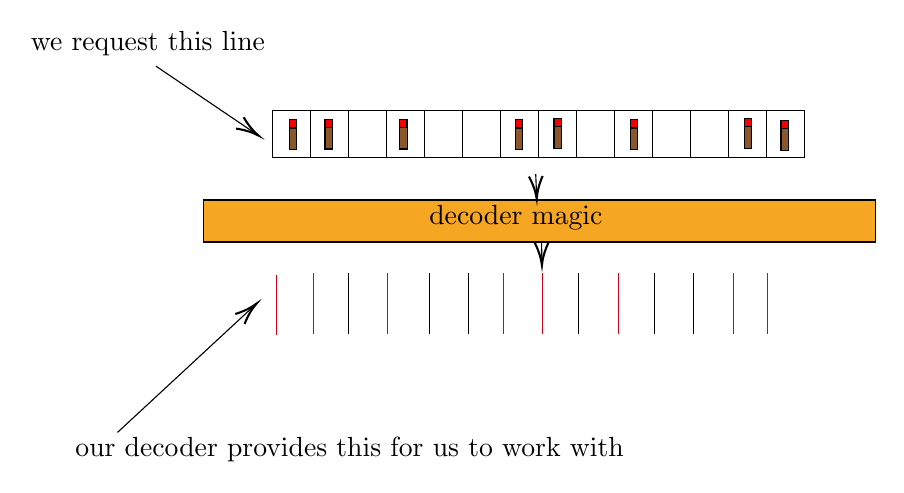
\begin{tikzpicture}[x=0.75pt,y=0.75pt,yscale=-1,xscale=1]
%uncomment if require: \path (0,300); %set diagram left start at 0, and has height of 300

%Shape: Rectangle [id:dp7306471770838919] 
\draw   (221,70.74) -- (239.33,70.74) -- (239.33,93.33) -- (221,93.33) -- cycle ;
%Shape: Rectangle [id:dp5607628345341253] 
\draw   (239.33,70.74) -- (257.67,70.74) -- (257.67,93.33) -- (239.33,93.33) -- cycle ;
%Shape: Rectangle [id:dp0792661956068278] 
\draw   (257.67,70.74) -- (276,70.74) -- (276,93.33) -- (257.67,93.33) -- cycle ;
%Shape: Rectangle [id:dp8623895262875295] 
\draw   (276,70.74) -- (294.33,70.74) -- (294.33,93.33) -- (276,93.33) -- cycle ;
%Shape: Rectangle [id:dp009175660727291923] 
\draw   (294.33,70.74) -- (312.67,70.74) -- (312.67,93.33) -- (294.33,93.33) -- cycle ;
%Shape: Rectangle [id:dp4729260459269564] 
\draw   (312.67,70.74) -- (331,70.74) -- (331,93.33) -- (312.67,93.33) -- cycle ;
%Shape: Rectangle [id:dp4530702176374507] 
\draw   (331,70.74) -- (349.33,70.74) -- (349.33,93.33) -- (331,93.33) -- cycle ;
%Shape: Rectangle [id:dp18274736433593486] 
\draw   (349.33,70.74) -- (367.67,70.74) -- (367.67,93.33) -- (349.33,93.33) -- cycle ;
%Shape: Rectangle [id:dp6454813939338947] 
\draw   (367.67,70.74) -- (386,70.74) -- (386,93.33) -- (367.67,93.33) -- cycle ;
%Shape: Rectangle [id:dp44415589930378796] 
\draw   (386,70.74) -- (404.33,70.74) -- (404.33,93.33) -- (386,93.33) -- cycle ;
%Shape: Rectangle [id:dp44316809627896814] 
\draw   (404.33,70.74) -- (422.67,70.74) -- (422.67,93.33) -- (404.33,93.33) -- cycle ;
%Shape: Rectangle [id:dp3768823609089883] 
\draw   (422.67,70.74) -- (441,70.74) -- (441,93.33) -- (422.67,93.33) -- cycle ;
%Shape: Rectangle [id:dp2370210201858336] 
\draw   (441,70.74) -- (459.33,70.74) -- (459.33,93.33) -- (441,93.33) -- cycle ;
%Shape: Rectangle [id:dp4899807962812457] 
\draw   (459.33,70.74) -- (477.67,70.74) -- (477.67,93.33) -- (459.33,93.33) -- cycle ;
%Shape: Rectangle [id:dp4368680678750193] 
\draw  [fill={rgb, 255:red, 139; green, 87; blue, 42 }  ,fill opacity=1 ] (229.17,79.08) -- (232.83,79.08) -- (232.83,89.5) -- (229.17,89.5) -- cycle ;
%Shape: Rectangle [id:dp09500539877263525] 
\draw  [fill={rgb, 255:red, 244; green, 0; blue, 0 }  ,fill opacity=1 ] (229.17,75.17) -- (232.67,75.17) -- (232.67,79.08) -- (229.17,79.08) -- cycle ;
%Shape: Rectangle [id:dp1483728050123183] 
\draw  [fill={rgb, 255:red, 139; green, 87; blue, 42 }  ,fill opacity=1 ] (246.5,78.75) -- (250.17,78.75) -- (250.17,89.17) -- (246.5,89.17) -- cycle ;
%Shape: Rectangle [id:dp593349582542728] 
\draw  [fill={rgb, 255:red, 244; green, 0; blue, 0 }  ,fill opacity=1 ] (246.5,74.83) -- (250,74.83) -- (250,78.75) -- (246.5,78.75) -- cycle ;
%Shape: Rectangle [id:dp4070158701487039] 
\draw  [fill={rgb, 255:red, 139; green, 87; blue, 42 }  ,fill opacity=1 ] (282.5,78.75) -- (286.17,78.75) -- (286.17,89.17) -- (282.5,89.17) -- cycle ;
%Shape: Rectangle [id:dp4458058453343535] 
\draw  [fill={rgb, 255:red, 244; green, 0; blue, 0 }  ,fill opacity=1 ] (282.5,74.83) -- (286,74.83) -- (286,78.75) -- (282.5,78.75) -- cycle ;
%Shape: Rectangle [id:dp9277371430125845] 
\draw  [fill={rgb, 255:red, 139; green, 87; blue, 42 }  ,fill opacity=1 ] (466.17,79.42) -- (469.83,79.42) -- (469.83,89.83) -- (466.17,89.83) -- cycle ;
%Shape: Rectangle [id:dp3082228602345055] 
\draw  [fill={rgb, 255:red, 244; green, 0; blue, 0 }  ,fill opacity=1 ] (466.17,75.5) -- (469.67,75.5) -- (469.67,79.42) -- (466.17,79.42) -- cycle ;
%Shape: Rectangle [id:dp17154116631501037] 
\draw  [fill={rgb, 255:red, 139; green, 87; blue, 42 }  ,fill opacity=1 ] (338.17,79.08) -- (341.83,79.08) -- (341.83,89.5) -- (338.17,89.5) -- cycle ;
%Shape: Rectangle [id:dp6278512827702475] 
\draw  [fill={rgb, 255:red, 244; green, 0; blue, 0 }  ,fill opacity=1 ] (338.17,75.17) -- (341.67,75.17) -- (341.67,79.08) -- (338.17,79.08) -- cycle ;
%Shape: Rectangle [id:dp31389089597210484] 
\draw  [fill={rgb, 255:red, 139; green, 87; blue, 42 }  ,fill opacity=1 ] (356.83,78.42) -- (360.5,78.42) -- (360.5,88.83) -- (356.83,88.83) -- cycle ;
%Shape: Rectangle [id:dp3848680259197699] 
\draw  [fill={rgb, 255:red, 244; green, 0; blue, 0 }  ,fill opacity=1 ] (356.83,74.5) -- (360.33,74.5) -- (360.33,78.42) -- (356.83,78.42) -- cycle ;
%Shape: Rectangle [id:dp6018543086688013] 
\draw  [fill={rgb, 255:red, 139; green, 87; blue, 42 }  ,fill opacity=1 ] (393.5,79.08) -- (397.17,79.08) -- (397.17,89.5) -- (393.5,89.5) -- cycle ;
%Shape: Rectangle [id:dp599252549604423] 
\draw  [fill={rgb, 255:red, 244; green, 0; blue, 0 }  ,fill opacity=1 ] (393.5,75.17) -- (397,75.17) -- (397,79.08) -- (393.5,79.08) -- cycle ;
%Shape: Rectangle [id:dp9476241971366911] 
\draw  [fill={rgb, 255:red, 139; green, 87; blue, 42 }  ,fill opacity=1 ] (448.5,78.42) -- (452.17,78.42) -- (452.17,88.83) -- (448.5,88.83) -- cycle ;
%Shape: Rectangle [id:dp6884535278941168] 
\draw  [fill={rgb, 255:red, 244; green, 0; blue, 0 }  ,fill opacity=1 ] (448.5,74.5) -- (452,74.5) -- (452,78.42) -- (448.5,78.42) -- cycle ;
%Straight Lines [id:da8130436103927301] 
\draw [color={rgb, 255:red, 208; green, 2; blue, 27 }  ,draw opacity=1 ]   (223,149.83) -- (223,178.83) ;
%Straight Lines [id:da08462131345193069] 
\draw [color={rgb, 255:red, 208; green, 2; blue, 27 }  ,draw opacity=1 ]   (241,149.17) -- (241,178.17) ;
%Straight Lines [id:da8359957829774382] 
\draw [color={rgb, 255:red, 208; green, 2; blue, 27 }  ,draw opacity=1 ]   (276.67,149.17) -- (276.67,178.17) ;
%Straight Lines [id:da3866920597345579] 
\draw [color={rgb, 255:red, 208; green, 2; blue, 27 }  ,draw opacity=1 ]   (332.67,149.17) -- (332.67,178.17) ;
%Straight Lines [id:da5942403939779883] 
\draw [color={rgb, 255:red, 208; green, 2; blue, 27 }  ,draw opacity=1 ]   (351.33,149.17) -- (351.33,178.17) ;
%Straight Lines [id:da22634310425539206] 
\draw [color={rgb, 255:red, 208; green, 2; blue, 27 }  ,draw opacity=1 ]   (388,149.17) -- (388,178.17) ;
%Straight Lines [id:da23791169110885224] 
\draw [color={rgb, 255:red, 208; green, 2; blue, 27 }  ,draw opacity=1 ]   (443.33,149.17) -- (443.33,178.17) ;
%Straight Lines [id:da9365841080673278] 
\draw [color={rgb, 255:red, 208; green, 2; blue, 27 }  ,draw opacity=1 ]   (459.67,149.17) -- (459.67,178.17) ;
%Straight Lines [id:da3945985170381383] 
\draw [color={rgb, 255:red, 0; green, 0; blue, 0 }  ,draw opacity=1 ]   (258,149.17) -- (258,178.17) ;
%Straight Lines [id:da3721123428333971] 
\draw [color={rgb, 255:red, 0; green, 0; blue, 0 }  ,draw opacity=1 ]   (297,149.17) -- (297,178.17) ;
%Straight Lines [id:da013616551740032623] 
\draw [color={rgb, 255:red, 0; green, 0; blue, 0 }  ,draw opacity=1 ]   (315.67,149.17) -- (315.67,178.17) ;
%Straight Lines [id:da9364095553547536] 
\draw [color={rgb, 255:red, 0; green, 0; blue, 0 }  ,draw opacity=1 ]   (368.67,149.17) -- (368.67,178.17) ;
%Straight Lines [id:da7903503951079389] 
\draw [color={rgb, 255:red, 0; green, 0; blue, 0 }  ,draw opacity=1 ]   (405.33,149.17) -- (405.33,178.17) ;
%Straight Lines [id:da6948026493349652] 
\draw [color={rgb, 255:red, 0; green, 0; blue, 0 }  ,draw opacity=1 ]   (424,149.17) -- (424,178.17) ;
%Straight Lines [id:da4088221703357503] 
\draw    (165,49.25) -- (212.84,81.63) ;
\draw [shift={(214.5,82.75)}, rotate = 214.09] [color={rgb, 255:red, 0; green, 0; blue, 0 }  ][line width=0.75]    (10.93,-3.29) .. controls (6.95,-1.4) and (3.31,-0.3) .. (0,0) .. controls (3.31,0.3) and (6.95,1.4) .. (10.93,3.29)   ;
%Straight Lines [id:da9371104688202003] 
\draw    (146.5,225.75) -- (212.03,165.03) ;
\draw [shift={(213.5,163.67)}, rotate = 497.18] [color={rgb, 255:red, 0; green, 0; blue, 0 }  ][line width=0.75]    (10.93,-3.29) .. controls (6.95,-1.4) and (3.31,-0.3) .. (0,0) .. controls (3.31,0.3) and (6.95,1.4) .. (10.93,3.29)   ;
%Shape: Rectangle [id:dp19839900197450522] 
\draw  [fill={rgb, 255:red, 245; green, 166; blue, 35 }  ,fill opacity=1 ] (188,113.75) -- (511.5,113.75) -- (511.5,134) -- (188,134) -- cycle ;
%Straight Lines [id:da7709890896181596] 
\draw    (348,101.25) -- (348.42,111.25) ;
\draw [shift={(348.5,113.25)}, rotate = 267.61] [color={rgb, 255:red, 0; green, 0; blue, 0 }  ][line width=0.75]    (10.93,-3.29) .. controls (6.95,-1.4) and (3.31,-0.3) .. (0,0) .. controls (3.31,0.3) and (6.95,1.4) .. (10.93,3.29)   ;
%Straight Lines [id:da6519792124694934] 
\draw    (350.83,133.67) -- (350.97,143.25) ;
\draw [shift={(351,145.25)}, rotate = 269.18] [color={rgb, 255:red, 0; green, 0; blue, 0 }  ][line width=0.75]    (10.93,-3.29) .. controls (6.95,-1.4) and (3.31,-0.3) .. (0,0) .. controls (3.31,0.3) and (6.95,1.4) .. (10.93,3.29)   ;

% Text Node
\draw (103.5,31) node [anchor=north west][inner sep=0.75pt]   [align=left] {we request this line};
% Text Node
\draw (125,227) node [anchor=north west][inner sep=0.75pt]   [align=left] {our decoder provides this for us to work with};
% Text Node
\draw (295.5,115) node [anchor=north west][inner sep=0.75pt]   [align=left] {decoder magic};


\end{tikzpicture}

    			
    		\end{frame}
    		
    		\begin{frame}
    			\frametitle{The Story So Far}
    			\begin{itemize}
    				\item Here's what we care about right now.
    			\end{itemize}
    			
    			

\tikzset{every picture/.style={line width=0.75pt}} %set default line width to 0.75pt        

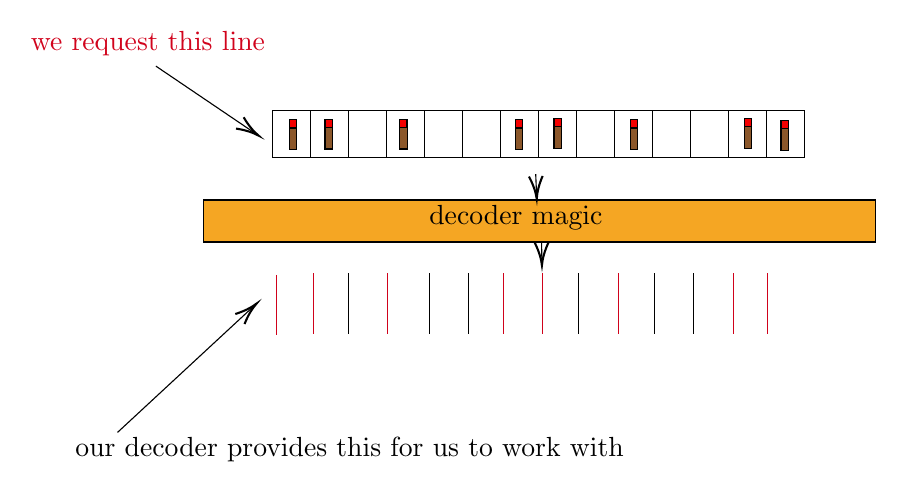
\begin{tikzpicture}[x=0.75pt,y=0.75pt,yscale=-1,xscale=1]
%uncomment if require: \path (0,300); %set diagram left start at 0, and has height of 300

%Shape: Rectangle [id:dp7306471770838919] 
\draw   (221,70.74) -- (239.33,70.74) -- (239.33,93.33) -- (221,93.33) -- cycle ;
%Shape: Rectangle [id:dp5607628345341253] 
\draw   (239.33,70.74) -- (257.67,70.74) -- (257.67,93.33) -- (239.33,93.33) -- cycle ;
%Shape: Rectangle [id:dp0792661956068278] 
\draw   (257.67,70.74) -- (276,70.74) -- (276,93.33) -- (257.67,93.33) -- cycle ;
%Shape: Rectangle [id:dp8623895262875295] 
\draw   (276,70.74) -- (294.33,70.74) -- (294.33,93.33) -- (276,93.33) -- cycle ;
%Shape: Rectangle [id:dp009175660727291923] 
\draw   (294.33,70.74) -- (312.67,70.74) -- (312.67,93.33) -- (294.33,93.33) -- cycle ;
%Shape: Rectangle [id:dp4729260459269564] 
\draw   (312.67,70.74) -- (331,70.74) -- (331,93.33) -- (312.67,93.33) -- cycle ;
%Shape: Rectangle [id:dp4530702176374507] 
\draw   (331,70.74) -- (349.33,70.74) -- (349.33,93.33) -- (331,93.33) -- cycle ;
%Shape: Rectangle [id:dp18274736433593486] 
\draw   (349.33,70.74) -- (367.67,70.74) -- (367.67,93.33) -- (349.33,93.33) -- cycle ;
%Shape: Rectangle [id:dp6454813939338947] 
\draw   (367.67,70.74) -- (386,70.74) -- (386,93.33) -- (367.67,93.33) -- cycle ;
%Shape: Rectangle [id:dp44415589930378796] 
\draw   (386,70.74) -- (404.33,70.74) -- (404.33,93.33) -- (386,93.33) -- cycle ;
%Shape: Rectangle [id:dp44316809627896814] 
\draw   (404.33,70.74) -- (422.67,70.74) -- (422.67,93.33) -- (404.33,93.33) -- cycle ;
%Shape: Rectangle [id:dp3768823609089883] 
\draw   (422.67,70.74) -- (441,70.74) -- (441,93.33) -- (422.67,93.33) -- cycle ;
%Shape: Rectangle [id:dp2370210201858336] 
\draw   (441,70.74) -- (459.33,70.74) -- (459.33,93.33) -- (441,93.33) -- cycle ;
%Shape: Rectangle [id:dp4899807962812457] 
\draw   (459.33,70.74) -- (477.67,70.74) -- (477.67,93.33) -- (459.33,93.33) -- cycle ;
%Shape: Rectangle [id:dp4368680678750193] 
\draw  [fill={rgb, 255:red, 139; green, 87; blue, 42 }  ,fill opacity=1 ] (229.17,79.08) -- (232.83,79.08) -- (232.83,89.5) -- (229.17,89.5) -- cycle ;
%Shape: Rectangle [id:dp09500539877263525] 
\draw  [fill={rgb, 255:red, 244; green, 0; blue, 0 }  ,fill opacity=1 ] (229.17,75.17) -- (232.67,75.17) -- (232.67,79.08) -- (229.17,79.08) -- cycle ;
%Shape: Rectangle [id:dp1483728050123183] 
\draw  [fill={rgb, 255:red, 139; green, 87; blue, 42 }  ,fill opacity=1 ] (246.5,78.75) -- (250.17,78.75) -- (250.17,89.17) -- (246.5,89.17) -- cycle ;
%Shape: Rectangle [id:dp593349582542728] 
\draw  [fill={rgb, 255:red, 244; green, 0; blue, 0 }  ,fill opacity=1 ] (246.5,74.83) -- (250,74.83) -- (250,78.75) -- (246.5,78.75) -- cycle ;
%Shape: Rectangle [id:dp4070158701487039] 
\draw  [fill={rgb, 255:red, 139; green, 87; blue, 42 }  ,fill opacity=1 ] (282.5,78.75) -- (286.17,78.75) -- (286.17,89.17) -- (282.5,89.17) -- cycle ;
%Shape: Rectangle [id:dp4458058453343535] 
\draw  [fill={rgb, 255:red, 244; green, 0; blue, 0 }  ,fill opacity=1 ] (282.5,74.83) -- (286,74.83) -- (286,78.75) -- (282.5,78.75) -- cycle ;
%Shape: Rectangle [id:dp9277371430125845] 
\draw  [fill={rgb, 255:red, 139; green, 87; blue, 42 }  ,fill opacity=1 ] (466.17,79.42) -- (469.83,79.42) -- (469.83,89.83) -- (466.17,89.83) -- cycle ;
%Shape: Rectangle [id:dp3082228602345055] 
\draw  [fill={rgb, 255:red, 244; green, 0; blue, 0 }  ,fill opacity=1 ] (466.17,75.5) -- (469.67,75.5) -- (469.67,79.42) -- (466.17,79.42) -- cycle ;
%Shape: Rectangle [id:dp17154116631501037] 
\draw  [fill={rgb, 255:red, 139; green, 87; blue, 42 }  ,fill opacity=1 ] (338.17,79.08) -- (341.83,79.08) -- (341.83,89.5) -- (338.17,89.5) -- cycle ;
%Shape: Rectangle [id:dp6278512827702475] 
\draw  [fill={rgb, 255:red, 244; green, 0; blue, 0 }  ,fill opacity=1 ] (338.17,75.17) -- (341.67,75.17) -- (341.67,79.08) -- (338.17,79.08) -- cycle ;
%Shape: Rectangle [id:dp31389089597210484] 
\draw  [fill={rgb, 255:red, 139; green, 87; blue, 42 }  ,fill opacity=1 ] (356.83,78.42) -- (360.5,78.42) -- (360.5,88.83) -- (356.83,88.83) -- cycle ;
%Shape: Rectangle [id:dp3848680259197699] 
\draw  [fill={rgb, 255:red, 244; green, 0; blue, 0 }  ,fill opacity=1 ] (356.83,74.5) -- (360.33,74.5) -- (360.33,78.42) -- (356.83,78.42) -- cycle ;
%Shape: Rectangle [id:dp6018543086688013] 
\draw  [fill={rgb, 255:red, 139; green, 87; blue, 42 }  ,fill opacity=1 ] (393.5,79.08) -- (397.17,79.08) -- (397.17,89.5) -- (393.5,89.5) -- cycle ;
%Shape: Rectangle [id:dp599252549604423] 
\draw  [fill={rgb, 255:red, 244; green, 0; blue, 0 }  ,fill opacity=1 ] (393.5,75.17) -- (397,75.17) -- (397,79.08) -- (393.5,79.08) -- cycle ;
%Shape: Rectangle [id:dp9476241971366911] 
\draw  [fill={rgb, 255:red, 139; green, 87; blue, 42 }  ,fill opacity=1 ] (448.5,78.42) -- (452.17,78.42) -- (452.17,88.83) -- (448.5,88.83) -- cycle ;
%Shape: Rectangle [id:dp6884535278941168] 
\draw  [fill={rgb, 255:red, 244; green, 0; blue, 0 }  ,fill opacity=1 ] (448.5,74.5) -- (452,74.5) -- (452,78.42) -- (448.5,78.42) -- cycle ;
%Straight Lines [id:da8130436103927301] 
\draw [color={rgb, 255:red, 208; green, 2; blue, 27 }  ,draw opacity=1 ]   (223,149.83) -- (223,178.83) ;
%Straight Lines [id:da08462131345193069] 
\draw [color={rgb, 255:red, 208; green, 2; blue, 27 }  ,draw opacity=1 ]   (241,149.17) -- (241,178.17) ;
%Straight Lines [id:da8359957829774382] 
\draw [color={rgb, 255:red, 208; green, 2; blue, 27 }  ,draw opacity=1 ]   (276.67,149.17) -- (276.67,178.17) ;
%Straight Lines [id:da3866920597345579] 
\draw [color={rgb, 255:red, 208; green, 2; blue, 27 }  ,draw opacity=1 ]   (332.67,149.17) -- (332.67,178.17) ;
%Straight Lines [id:da5942403939779883] 
\draw [color={rgb, 255:red, 208; green, 2; blue, 27 }  ,draw opacity=1 ]   (351.33,149.17) -- (351.33,178.17) ;
%Straight Lines [id:da22634310425539206] 
\draw [color={rgb, 255:red, 208; green, 2; blue, 27 }  ,draw opacity=1 ]   (388,149.17) -- (388,178.17) ;
%Straight Lines [id:da23791169110885224] 
\draw [color={rgb, 255:red, 208; green, 2; blue, 27 }  ,draw opacity=1 ]   (443.33,149.17) -- (443.33,178.17) ;
%Straight Lines [id:da9365841080673278] 
\draw [color={rgb, 255:red, 208; green, 2; blue, 27 }  ,draw opacity=1 ]   (459.67,149.17) -- (459.67,178.17) ;
%Straight Lines [id:da3945985170381383] 
\draw [color={rgb, 255:red, 0; green, 0; blue, 0 }  ,draw opacity=1 ]   (258,149.17) -- (258,178.17) ;
%Straight Lines [id:da3721123428333971] 
\draw [color={rgb, 255:red, 0; green, 0; blue, 0 }  ,draw opacity=1 ]   (297,149.17) -- (297,178.17) ;
%Straight Lines [id:da013616551740032623] 
\draw [color={rgb, 255:red, 0; green, 0; blue, 0 }  ,draw opacity=1 ]   (315.67,149.17) -- (315.67,178.17) ;
%Straight Lines [id:da9364095553547536] 
\draw [color={rgb, 255:red, 0; green, 0; blue, 0 }  ,draw opacity=1 ]   (368.67,149.17) -- (368.67,178.17) ;
%Straight Lines [id:da7903503951079389] 
\draw [color={rgb, 255:red, 0; green, 0; blue, 0 }  ,draw opacity=1 ]   (405.33,149.17) -- (405.33,178.17) ;
%Straight Lines [id:da6948026493349652] 
\draw [color={rgb, 255:red, 0; green, 0; blue, 0 }  ,draw opacity=1 ]   (424,149.17) -- (424,178.17) ;
%Straight Lines [id:da4088221703357503] 
\draw    (165,49.25) -- (212.84,81.63) ;
\draw [shift={(214.5,82.75)}, rotate = 214.09] [color={rgb, 255:red, 0; green, 0; blue, 0 }  ][line width=0.75]    (10.93,-3.29) .. controls (6.95,-1.4) and (3.31,-0.3) .. (0,0) .. controls (3.31,0.3) and (6.95,1.4) .. (10.93,3.29)   ;
%Straight Lines [id:da9371104688202003] 
\draw    (146.5,225.75) -- (212.03,165.03) ;
\draw [shift={(213.5,163.67)}, rotate = 497.18] [color={rgb, 255:red, 0; green, 0; blue, 0 }  ][line width=0.75]    (10.93,-3.29) .. controls (6.95,-1.4) and (3.31,-0.3) .. (0,0) .. controls (3.31,0.3) and (6.95,1.4) .. (10.93,3.29)   ;
%Shape: Rectangle [id:dp19839900197450522] 
\draw  [fill={rgb, 255:red, 245; green, 166; blue, 35 }  ,fill opacity=1 ] (188,113.75) -- (511.5,113.75) -- (511.5,134) -- (188,134) -- cycle ;
%Straight Lines [id:da7709890896181596] 
\draw    (348,101.25) -- (348.42,111.25) ;
\draw [shift={(348.5,113.25)}, rotate = 267.61] [color={rgb, 255:red, 0; green, 0; blue, 0 }  ][line width=0.75]    (10.93,-3.29) .. controls (6.95,-1.4) and (3.31,-0.3) .. (0,0) .. controls (3.31,0.3) and (6.95,1.4) .. (10.93,3.29)   ;
%Straight Lines [id:da6519792124694934] 
\draw    (350.83,133.67) -- (350.97,143.25) ;
\draw [shift={(351,145.25)}, rotate = 269.18] [color={rgb, 255:red, 0; green, 0; blue, 0 }  ][line width=0.75]    (10.93,-3.29) .. controls (6.95,-1.4) and (3.31,-0.3) .. (0,0) .. controls (3.31,0.3) and (6.95,1.4) .. (10.93,3.29)   ;

% Text Node
\draw (103.5,31) node [anchor=north west][inner sep=0.75pt]   [align=left] {\textcolor[rgb]{0.82,0.01,0.11}{we request this line}};
% Text Node
\draw (125,227) node [anchor=north west][inner sep=0.75pt]   [align=left] {our decoder provides this for us to work with};
% Text Node
\draw (295.5,115) node [anchor=north west][inner sep=0.75pt]   [align=left] {decoder magic};


\end{tikzpicture}

    			

    			
    		\end{frame}
    	
	\subsection{What we need}    	
    	
    	\begin{frame}
    		\frametitle{Requirements}
    		\begin{itemize}
    			\item So we know that we need a way to \textbf{request lines}.
    			\item We also know that such a request has to be input in \textbf{binary}.
    			\item \textit{If you don't know this already, make sure you know why.}
    		\end{itemize}
    	\end{frame}
    	
    	\begin{frame}
    		\frametitle{Sequentiality}
    		\begin{itemize}
    			\item Ok, let's think about the \textbf{order} in which we request them
    			\item After all, after we request one line, we're going to need a way to request the next.
    			\begin{itemize}
    				\item Then the next after that, then the next after that, etc.
    			\end{itemize}
    			\item This is where the idea of sequential logic comes in.
    		\end{itemize}
    	\end{frame}
    	
    	\begin{frame}
    		\frametitle{Sequentiality}
    		\begin{itemize}
    			\item And, we aren't just thinking in terms of moving one by one.
    			\item After all, is 1 the only amount we're ever going to be incrementing by?
    			\item What about statements like \texttt{BRANCHEQ} in our 389E Assembly? How will we handle that?
    			
    		\end{itemize}
    	\end{frame}
    	
    	\begin{frame}
    		\frametitle{Requirements}
    		\begin{itemize}
    			\item Let's not get too confused with it all right now, we're just outlining specifications
    			\item We've pondered enough, let's quantify our goals
    			\begin{itemize}
    				\item What we've \textbf{got so far}
    				\item What we \textbf{need}
    			\end{itemize}
    			
    		\end{itemize}
    	\end{frame}
    	
    	\begin{frame}
    		\frametitle{So What've We Got?}
    		\begin{itemize}
    			\item Excellent ROM Architecture that takes in a \textbf{binary number} as a signal and produces the corresponding \textbf{line of code}
    		\end{itemize}
    	\end{frame}
    	
    	\begin{frame}
    		\frametitle{What Do We Need?}
    		\begin{itemize}
    			\item We need a circuit that produces \textbf{line numbers} in \textbf{binary}.
    			\item It needs to work \textbf{sequentially} (Produce a signal for 1, then 2, then 3, etc.)
    			\item Additionally, it needs to be able to handle \texttt{BRANCHEQ} as well.
    			\begin{itemize}
    				\item That is, it needs to be able to \textbf{increment and decrement by arbitrary quantities}, i.e. \textbf{jump} from one line to another.
    				\item For example, if we needed to 'jump' from line 2 to 5, this could be handled by incrementing our counter by 3.
    			\end{itemize}
    		\end{itemize}
    	\end{frame}
    		     	
    		     	
    	\begin{frame}
    		\frametitle{In Relation To..}
    		\begin{itemize}
    			\item Here's where our new circuit will belong among our other planned components. Again, we're working on the orange one.
    		\end{itemize}
    		
    		{
    		\centering
    		

\tikzset{every picture/.style={line width=0.75pt}} %set default line width to 0.75pt        

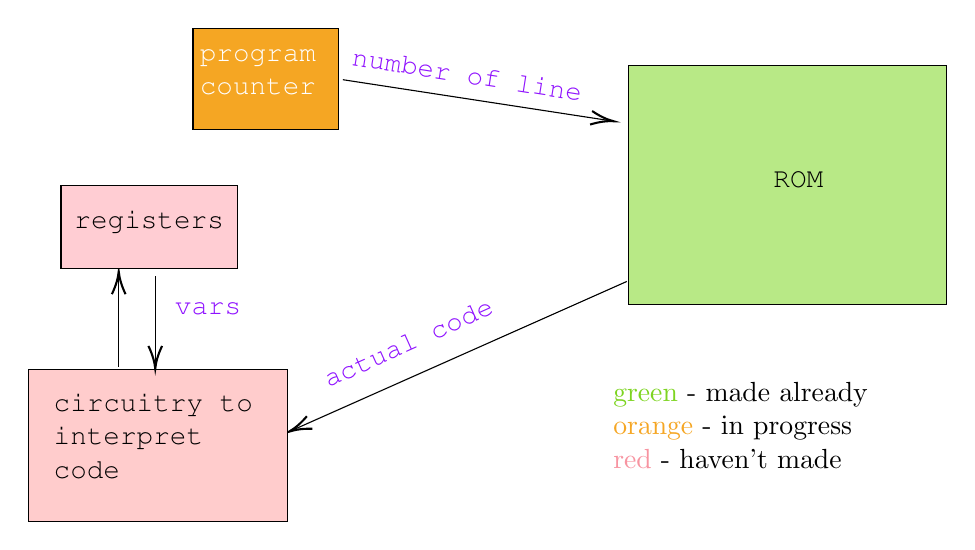
\begin{tikzpicture}[x=0.75pt,y=0.75pt,yscale=-1,xscale=1]
%uncomment if require: \path (0,300); %set diagram left start at 0, and has height of 300

%Shape: Rectangle [id:dp5921038974610358] 
\draw  [fill={rgb, 255:red, 184; green, 233; blue, 134 }  ,fill opacity=1 ] (308.4,56.6) -- (461.4,56.6) -- (461.4,172) -- (308.4,172) -- cycle ;
%Shape: Rectangle [id:dp7682132847374952] 
\draw  [fill={rgb, 255:red, 245; green, 166; blue, 35 }  ,fill opacity=1 ] (98.4,38.8) -- (168.4,38.8) -- (168.4,87.6) -- (98.4,87.6) -- cycle ;
%Straight Lines [id:da4338022631406676] 
\draw    (170.6,63.6) -- (299.02,83.3) ;
\draw [shift={(301,83.6)}, rotate = 188.72] [color={rgb, 255:red, 0; green, 0; blue, 0 }  ][line width=0.75]    (10.93,-3.29) .. controls (6.95,-1.4) and (3.31,-0.3) .. (0,0) .. controls (3.31,0.3) and (6.95,1.4) .. (10.93,3.29)   ;
%Straight Lines [id:da6665272072032727] 
\draw    (307.4,160.8) -- (146.43,232.39) ;
\draw [shift={(144.6,233.2)}, rotate = 336.02] [color={rgb, 255:red, 0; green, 0; blue, 0 }  ][line width=0.75]    (10.93,-3.29) .. controls (6.95,-1.4) and (3.31,-0.3) .. (0,0) .. controls (3.31,0.3) and (6.95,1.4) .. (10.93,3.29)   ;
%Shape: Rectangle [id:dp27632518285076746] 
\draw  [fill={rgb, 255:red, 255; green, 204; blue, 204 }  ,fill opacity=1 ] (19,203.2) -- (143.8,203.2) -- (143.8,276.4) -- (19,276.4) -- cycle ;
%Straight Lines [id:da9669220764176485] 
\draw    (62.6,202) -- (62.6,158) ;
\draw [shift={(62.6,156)}, rotate = 450] [color={rgb, 255:red, 0; green, 0; blue, 0 }  ][line width=0.75]    (10.93,-3.29) .. controls (6.95,-1.4) and (3.31,-0.3) .. (0,0) .. controls (3.31,0.3) and (6.95,1.4) .. (10.93,3.29)   ;
%Straight Lines [id:da14482572171663322] 
\draw    (80.2,158.4) -- (80.2,200.8) ;
\draw [shift={(80.2,202.8)}, rotate = 270] [color={rgb, 255:red, 0; green, 0; blue, 0 }  ][line width=0.75]    (10.93,-3.29) .. controls (6.95,-1.4) and (3.31,-0.3) .. (0,0) .. controls (3.31,0.3) and (6.95,1.4) .. (10.93,3.29)   ;
%Shape: Rectangle [id:dp8111716839726016] 
\draw  [fill={rgb, 255:red, 255; green, 205; blue, 211 }  ,fill opacity=1 ] (34.8,114.4) -- (119.8,114.4) -- (119.8,154.4) -- (34.8,154.4) -- cycle ;

% Text Node
\draw (100.4,47.6) node [anchor=north west][inner sep=0.75pt]   [align=left] {{\fontfamily{pcr}\selectfont \textcolor[rgb]{1,1,1}{program}}\\{\fontfamily{pcr}\selectfont \textcolor[rgb]{1,1,1}{counter}}};
% Text Node
\draw (376.8,106.4) node [anchor=north west][inner sep=0.75pt]   [align=left] {{\fontfamily{pcr}\selectfont ROM}};
% Text Node
\draw (174.9,46.35) node [anchor=north west][inner sep=0.75pt]  [color={rgb, 255:red, 144; green, 19; blue, 254 }  ,opacity=1 ,rotate=-9] [align=left] {{\fontfamily{pcr}\selectfont number of line}};
% Text Node
\draw (158.43,203.75) node [anchor=north west][inner sep=0.75pt]  [rotate=-335.85] [align=left] {{\fontfamily{pcr}\selectfont \textcolor[rgb]{0.56,0.07,1}{actual code}}\\};
% Text Node
\draw (30,213.4) node [anchor=north west][inner sep=0.75pt]   [align=left] {{\fontfamily{pcr}\selectfont circuitry to}\\{\fontfamily{pcr}\selectfont interpret}\\{\fontfamily{pcr}\selectfont code}};
% Text Node
\draw (40,125.4) node [anchor=north west][inner sep=0.75pt]   [align=left] {{\fontfamily{pcr}\selectfont registers}};
% Text Node
\draw (88.4,169.8) node [anchor=north west][inner sep=0.75pt]   [align=left] {{\fontfamily{pcr}\selectfont \textcolor[rgb]{0.56,0.07,1}{vars}}};
% Text Node
\draw (299.6,208.2) node [anchor=north west][inner sep=0.75pt]   [align=left] {\textcolor[rgb]{0.49,0.83,0.13}{green} - made already\\\textcolor[rgb]{0.96,0.65,0.14}{orange} - in progress\\\textcolor[rgb]{0.97,0.58,0.63}{red} - haven't made};


\end{tikzpicture}

    		}
    	\end{frame}

       
             
            
        
   	
\end{document}
